\begin{figure*}[tbh] 
\vspace{-0. in}
\centering
\centerline{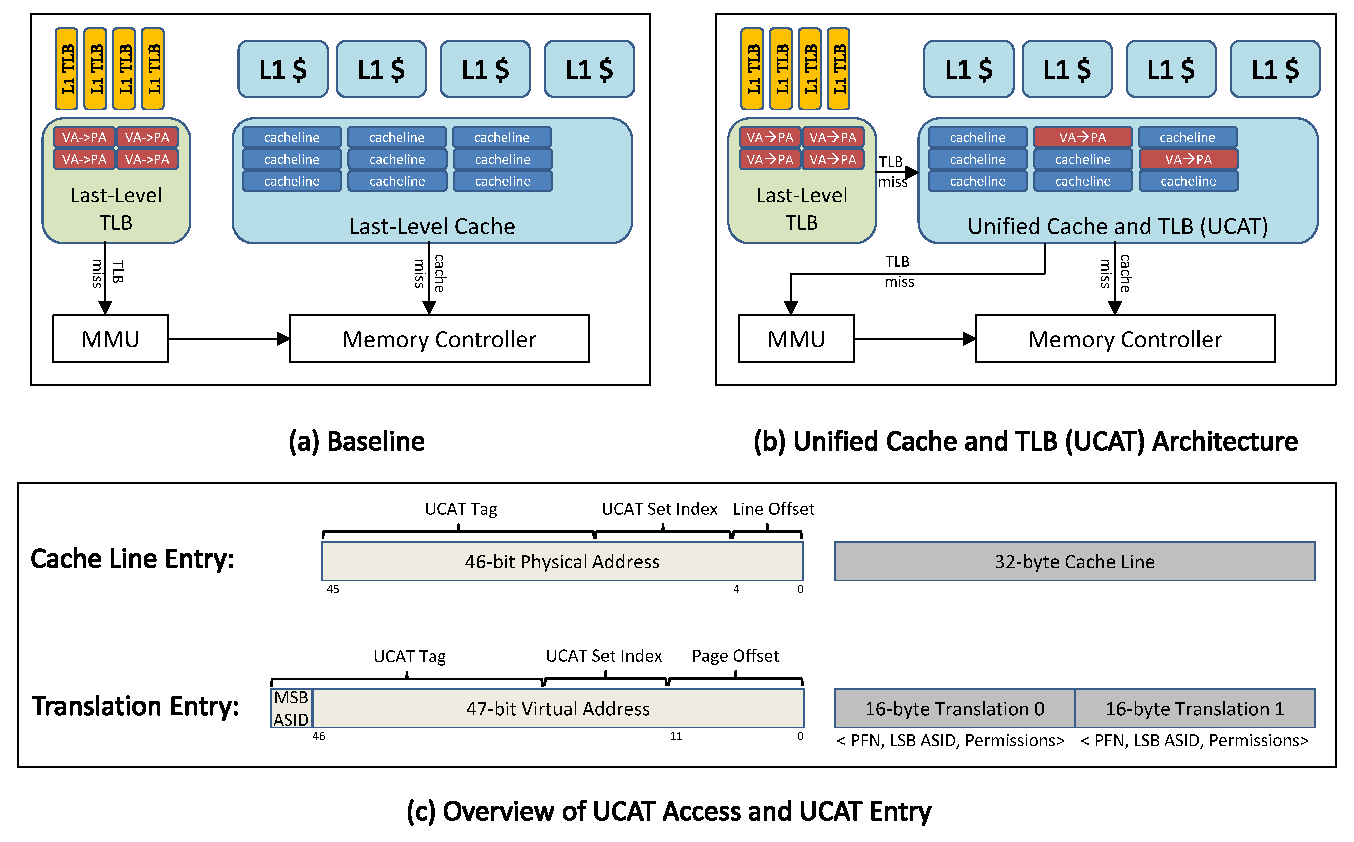
\psfig{file=FIGURES/UCAT,scale=0.80,width=\textwidth}}
\caption{\small UCAT Architecture. \normalsize}
\label{fig:UCAT} 
\vspace{-0.0in}
\end{figure*}

\section{Unifying Caches and TLBs}
\label{sec:UCAT}

\noindent Modern chip multiprocessors use multi-level TLB and cache
hierarchies for high performance. The last-level in each hierarchy is
architected as a single large unified structure that holds both
instruction and data entries and is shared among all cores. For
example, the unified last-level cache (LLC) contains hundreds of
thousands of cache lines (e.g., 256k lines in an 8MB cache with 32B
cache lines). Similarly, the unified last-level TLB (LLT) contains
512-1024 TLB entries~\cite{sodani2016knights,ia_manual}.

% that store data for recent memory references.
% that store address translations for recent memory references.

The LLT and LLC are cache structures with a tag array and a data
array. The LLT tag array stores virtual addresses while the LLC tag
array stores physical addresses\footnote{Additional meta data (e.g.,
coherence state, replacement state, etc.) is also stored in the tag
array.}. The LLT data array stores the physical address corresponding
to the virtual address translation (roughly 8 bytes), while the LLC
data array stores a copy of the data from memory at a cache line
granularity (e.g., 32-64 bytes).


%EIMAN-03-21: verify that each LLC line can indeed hold one LLT entry.

The LLT and LLC have similar sized tag arrays. However, since they
provide different types of data, the LLC has a 4x-8x larger data
array. To increase on-die LLT capacity, we observe that the LLC can
potentially also serve as gigantic TLB with as many entries as there
are LLC lines. Given that LLCs typically have low hit-rates and are
often inefficiently
used~\cite{jaleel_rrip,setdueling,wu2011,jimenez_micro2013,khan2010},
the conventional LLC can be used to store virtual to physical
translations just like a TLB (in addition to caching data from
memory). Based on this insight, we re-architect the conventional LLC
as a {\em Unified Cache and TLB (UCAT)}.

%EIMAN-03-21: My summary for reworking later: 
%   - both TLB and cache hierarchies involve multiple levels and many entries in the unified LL
%   - there is a distinction between what the tag and data of each hierarhcy holds but the cache data portion is bigger
%   - Since the tag arrays are similar in size (does this even matter?), we think of using part of the larger part of the data array of the caches to hold translation entries?
%   - Could the motivaiton here at the end be done better? Isn't the motivation really that the LLC space isn't very efficiently used in the GPU, and its the GPU translations that we care about based on the citation that we had in the intro, right?

\subsection{UCAT Architecture}

\noindent Figure~\ref{fig:UCAT}(a) illustrates a baseline system with
separate LLT and LLC structures, while Figure~\ref{fig:UCAT}(b)
demonstrates a system with a separate LLT and a Unified Cache and TLB
(UCAT). In the latter system, the UCAT holds both cache lines and TLB
entries in a single hardware structure. Figure~\ref{fig:UCAT}(c) shows
how this is done. When a UCAT entry stores a cache line similar to
what the baseline system does, the tag-array stores a portion of the
physical address while the data array stores the cache line (e.g.,
32-bytes)\footnote{In our baseline we assume a physically indexed,
physically tagged cache. However, any other variant of virtual or
physical indexing/tagging is equally possible with UCAT.}. However,
when the UCAT entry serves as a TLB entry, the UCAT tag-array stores
portions of the virtual address and the address space identifier
(ASID), while the data-array stores the virtual to physical address
translation, and additional information such as page protection bits,
and possibly some ASID bits. Storing some ASID bits in the data array
may be necessary if all the ASID bits do not fit in the existing LLC
tag array size. In such situations, we propose to store the top bits
of the ASID in the tag array. This enables a partial tag match and
avoids false positives when multiple programs with identical virtual
addresses concurrently execute. Note that the bottom bits of the ASID
(stored in the data array) must be compared for a match before
supplying the translation stored in the UCAT-entry. We use 16 bytes of
the UCAT data array for storing the address translation.

Even though we only use 16-bytes of the 32-byte line to store the
translation, UCAT improves upon the existing LLC inefficiency. This is
because recent studies show (and this study independently verifies)
that the majority of LLC entries are unused after cache
insertion~\cite{jaleel_rrip,setdueling,wu2011,jimenez_micro2013,khan2010}.
As such, UCAT utilizes the conventional LLC space more efficiently by
storing TLB entries in addition to cache lines. Note that UCAT space
efficiency can be improved further by compressing multiple TLB entries
into the data array. However, we leave these optimizations for future
work.

In the UCAT design, cache lines and TLB-entries dynamically contend for
the available UCAT space. Like the baseline LLC architecture, we
leverage the existing replacement policy to manage allocating UCAT
entries in a set. UCAT hits update replacement state while UCAT misses
utilize the baseline replacement policy to select the victim.

The baseline UCAT replacement policy allocates entries based on
demand, rather than utility. This can potentially create performance
problems in TLB-sensitive workloads that frequently stream through a
large number of cache lines and constantly discard performance critical
UCAT TLB entries. Based on this insight, we enhance the baseline UCAT
design by improving the replacement policy. To this end, we
leverage the Dynamic Re-Reference Interval Prediction (DRRIP)
replacement policy~\cite{jaleel_rrip}. In this policy, all UCAT
insertions follow the same re-reference prediction or insertion
policy. We propose enhancing the insertion policy for TLB entries by
inserting them with a {\em near-immediate prediction} rather than the
default {\em far prediction}. By doing so, TLB entries reside in the
UCAT for a longer duration. We refer to this enhancement as {\em UCAT
with Insertion (UCAT-I)}.

% \subsection{Static UCAT Partitioning}
% 
% \noindent UCAT entries must be distributed between TLB-entries and
% cachelines. One way of accomplishing this is by statically employing
% {\em way partitioning}~\cite{}. With {\em N} ways in a UCAT set, {\em
% m} ways are statically devoted to cachelines while the remaining {\em
% N-m} ways are statically devoted to TLB entries. Cachelines are only
% inserted in the ways to devoted to them while TLB entries are inserted
% in the ways devoted to them. When evicting UCAT entries, a replacement
% policy is used (e.g. LRU, RRIP) to select between candidates within
% the same UCAT partition. We refer to this design as {\em Static UCAT
% Partitioning (UCAT-S)}.
% 
% Profiling across various workloads for different values of {\em m} can
% help arrive at the best UCAT partition for cachelines and TLB entries.
% Figure X illustrates the behavior for different {\em m}.

\subsection{UCAT Performance}

% PUCAT is inefficient when the TLB-entries and cachelines have
% different capacity requirements at run time. To address this problen,

\noindent Figure~\ref{fig:perf_UCAT} shows UCAT performance relative
to the baseline system(on the y-axis) with workloads on the x-axis.
The first bar in the figure shows UCAT performance where cache lines
and TLB-entries contend for UCAT space without any restrictions. The
figure shows that UCAT significantly improves performance of workloads
like {\em XSBench}, {\em dmr}, {\em MaxFlow}, and {\em MCB} by more
than 2x (up to 4x in the latter two). Other workloads like {\em GUPS},
{\em SNAP}, {\em UMT}, and {\em CoMD} observe more than 15\%
performance gains. Overall, UCAT improves performance across all
workloads by 53\%.

To understand the performance benefits of UCAT,
Figure~\ref{fig:tlblat_UCAT} and Figure~\ref{fig:tlbsize_UCAT}
illustrate relative translation latency and effective on-die TLB size
respectively. The effective on-die TLB size is reported as the average
number of TLB entries in the UCAT (sampled every 10 million cycles)
during the course of application execution.

Workloads with more than 2x performance improvements observe a
reduction in TLB miss penalty by 70\% or more. This is because these
workloads experience an increase in on-die TLB size of 4x-64x. On
average, UCAT improves virtual to physical address translation latency
by 51\% (up to 86\% for {\em MCB}). The improvement in translation
latency stems from an increase in on-chip TLB coverage by 16x (up to
64x for {\em dmr}).

\begin{figure}[tp] 
  \vspace{-0.in} \centering
  \centerline{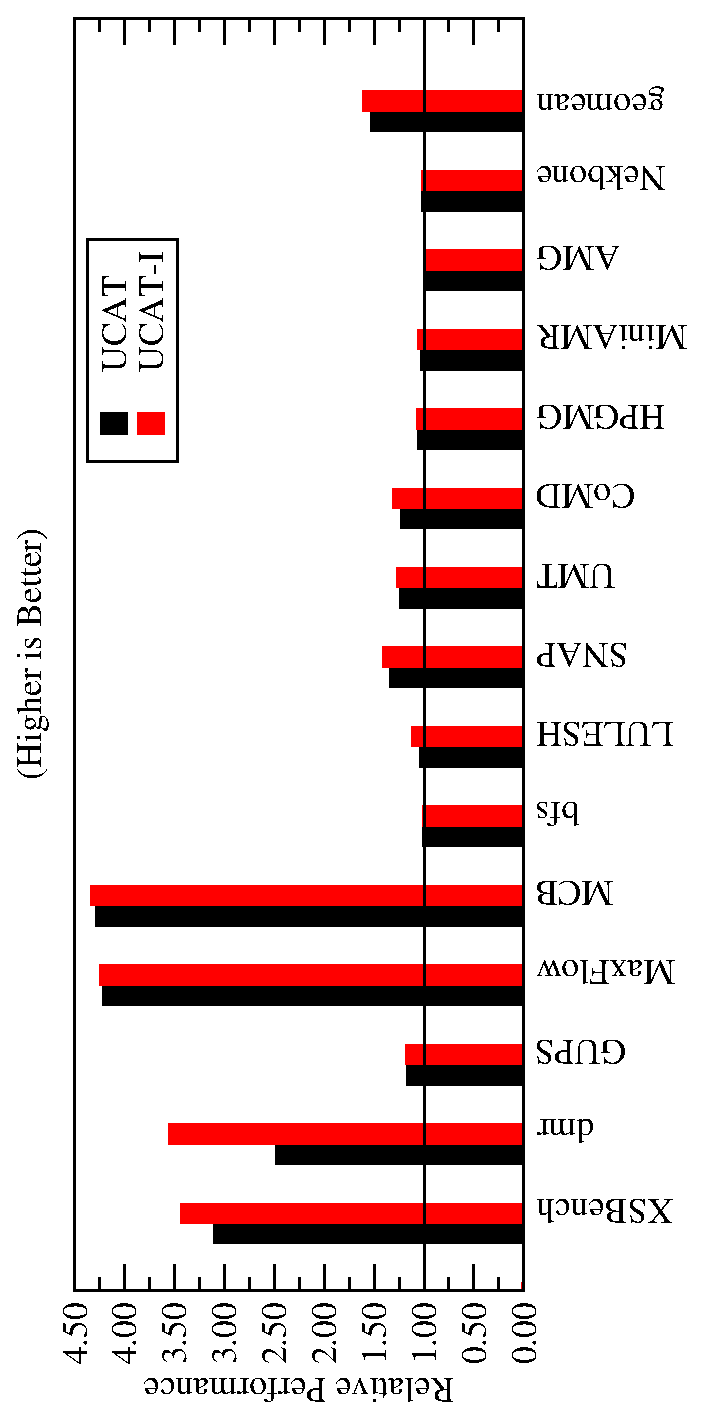
\psfig{file=GRAPHS/UCAT_perf,angle=-90,width=\columnwidth}}

  \caption{\small UCAT Performance. \normalsize}
  \label{fig:perf_UCAT} 
  \vspace{0.1 in}
\end{figure}

\begin{figure}[tp] 
  \vspace{0.1in} \centering
  \centerline{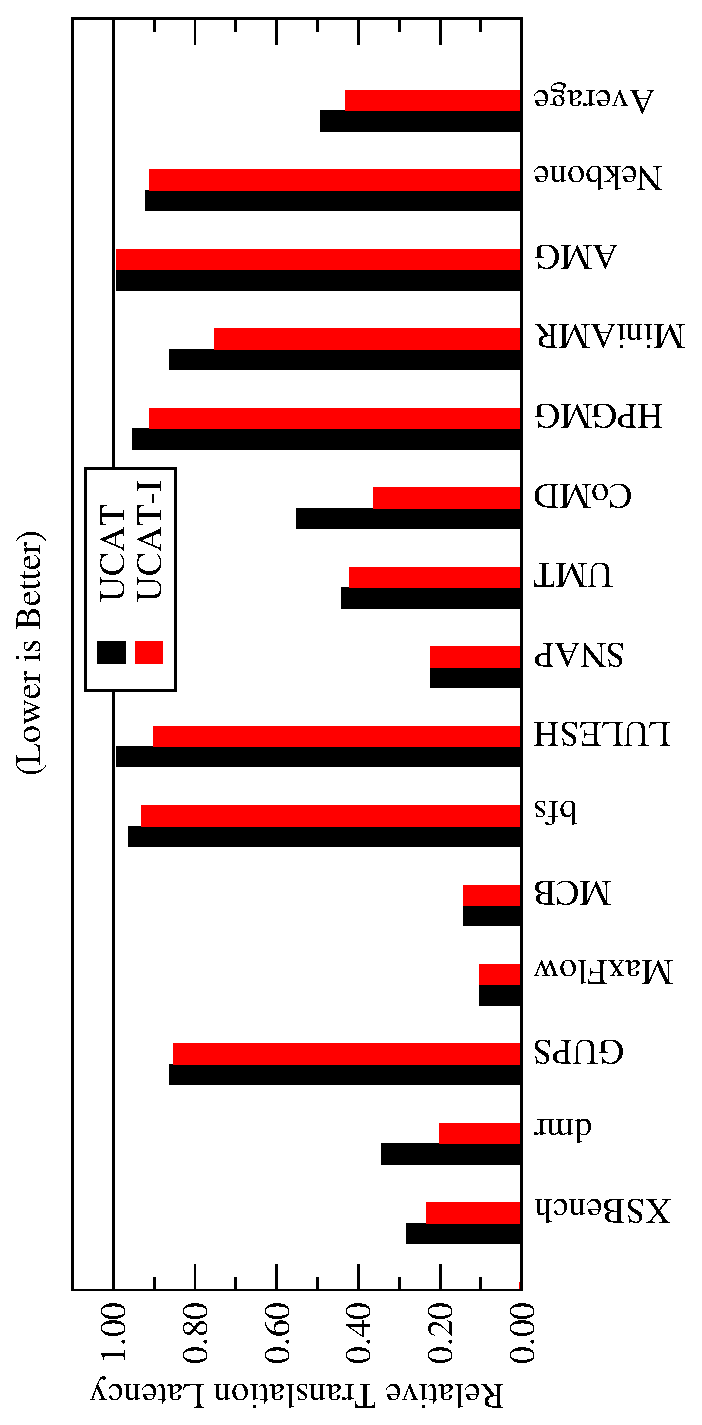
\psfig{file=GRAPHS/UCAT_tlblat,angle=-90,width=\columnwidth}}

  \caption{\small Relative Translation latency.\normalsize}
  \label{fig:tlblat_UCAT} 
  \vspace{-0.0 in}
\end{figure}

\begin{figure}[b]
  \vspace{0.2in} \centering
  \centerline{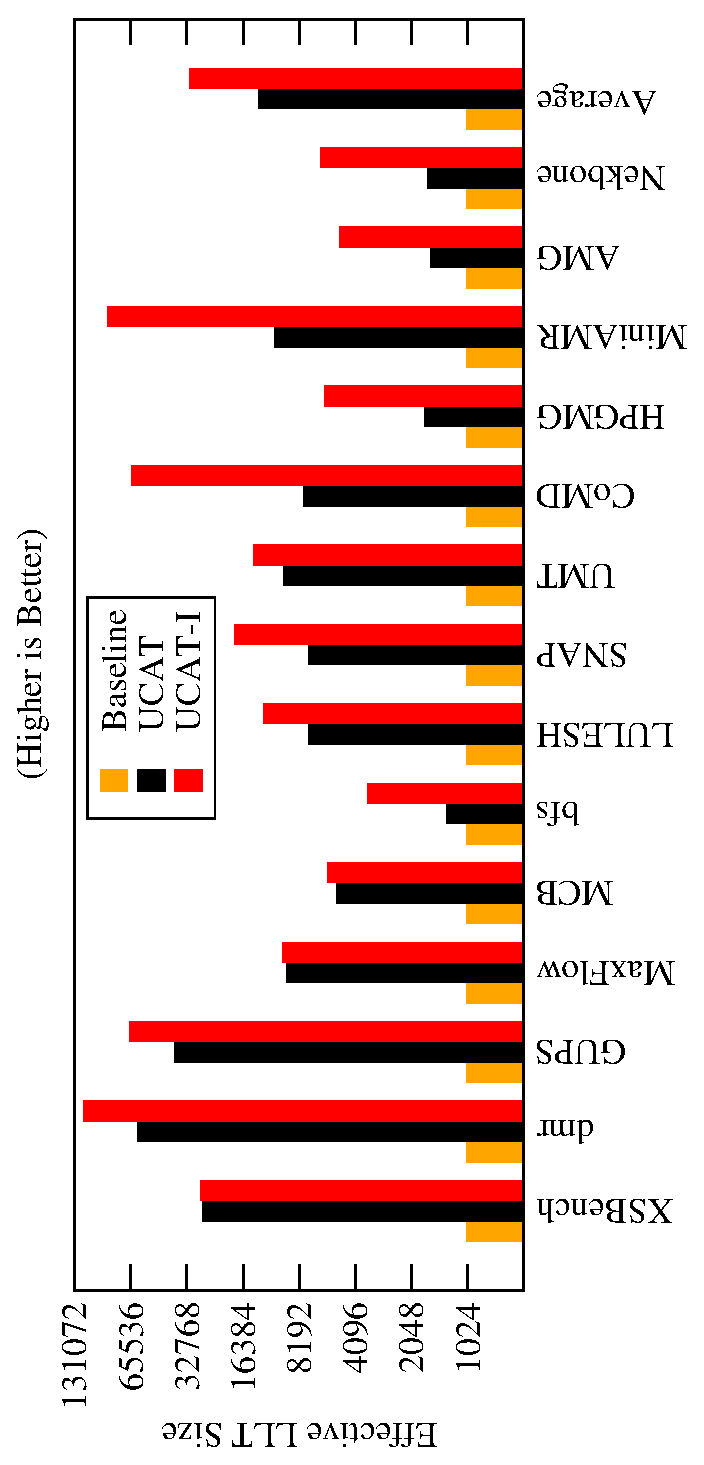
\psfig{file=GRAPHS/UCAT_tlbsize,angle=-90,width=\columnwidth}}

  \caption{\small Effective On-Die TLB Size with UCAT.\normalsize}
  \label{fig:tlbsize_UCAT} 
  \vspace{-0.0 in}
\end{figure}

Since UCAT decreases the effective capacity of cache lines compared to
the separate LLC, we investigated the increase in memory traffic
relative to the baseline design. Our evaluations show that on average,
UCAT increases the number of memory accesses by 1\% (maximum 4\% for
{\em XSBench}). As observed from the performance graphs, the
additional increase in memory traffic has negligible performance
impact. This illustrates that trading off conventional LLC space for
TLB entries provides substantial performance improvements.

Figure~\ref{fig:perf_UCAT} also shows that intelligently managing UCAT
by prioritizing TLB-entries over cache lines improves average UCAT
performance by an additional 12\%. We observed that UCAT-I also has
negligible increase in memory traffic (< 1\%) and TLB-sensitive
workloads like {\em XSBench} and {\em dmr} experience additional
performance improvements of up to 90\%. Additionally, workloads like
{\em LULESH}, {\em SNAP}, and {\em CoMD} experience an additional
7-10\% performance improvement over UCAT by intelligently managing the
UCAT-entries. This is evident from Figures~\ref{fig:tlblat_UCAT}
and~\ref{fig:tlbsize_UCAT} where UCAT-I increases effective TLB
coverage by nearly 2x while improving average translation latency by
7\%. Overall, UCAT-I improves performance by 65\% relative to the
baseline.

\subsection{UCAT Design Overhead}

\noindent UCAT requires a mechanism to distinguish between cacheline
entries and translation entries. We propose using the UCAT-entry state
bits (i.e., MESI bits) and insert TLB-entries into UCAT with the {\em
exclusive} and {\em shared} status bits both set to valid. Since cache
lines can either be in exclusive state or shared state and not both,
this proposal enables distinguishing between TLB entries and cacheline
entries at zero storage overhead. Besides distinguishing between
cacheline and translation entries, UCAT also requires efficient
support for handling TLB shootdown and TLB flush requests. We discuss
these design issues in Section~\ref{sec:implications}.

%<<<<<<< HEAD
%UCAT requires additional logic to invalidate/flush TLB entries from
%the UCAT. Targeted virtual address invalidations can be handled by
%looking up and invalidating the UCAT-entry. However, to enable a TLB
%flush for a given ASID, an 8-bit {\em Epoch Counter (EPCTR)} can be
%associated with each ASID. When inserting a TLB-entry into UCAT,
%besides storing the physical address and permission bits, the current
%value of the EPCTR for the ASID is also stored. If the ASID requires a
%TLB flush, the EPCTR can be incremented. With such support, UCAT
%provides a valid translation only if both the ASID and EPCTR stored in
%the UCAT-entry match the current EPCTR for the ASID corresponding to a memory request.
%=======
% UCAT requires additional logic to invalidate/flush TLB entries from
% the UCAT. Targeted virtual address invalidations can be handled by
% looking up and invalidating the UCAT-entry. 
%>>>>>>> 260a7f3bf4840016bd190ffb4d24f59bad2e373f
